% use paper, or submit
% use 11 pt (preferred), 12 pt, or 10 pt only

\documentclass[letterpaper, paper,11pt]{./AAS}		% for final proceedings (20-page limit)

\usepackage{bm}
\usepackage{amsmath}
\usepackage{subfigure}
\usepackage[colorlinks=true, pdfstartview=FitV, linkcolor=black, citecolor= black, urlcolor= black]{hyperref}
\usepackage{xfrac}
\usepackage{booktabs}

\begin{document}

\subsection{$\Delta V$EGA Maneuver Implementation}
A $\Delta V$EGA orbit, also referred to as a leveraging orbit specifically of Earth, launches with the intent to gravity assist off the body for a higher post-flyby heliocentric energy\cite{Hollenbeck}.  Leveraging orbits are classified by their nominal resonance period multiple with respect to the flyby body's heliocentric orbit, and we will refer to this number as "$k$." For example, a leveraging orbit that has a period roughly 3 times as large as Earth's will have a $k=3$ which is represented as a 3:1 $\Delta V$EGA trajectory. The actual period of these orbits will vary either greater than or less than the nominal time due to flying by the body at a different Earth heliocentric true anomaly. Trajectories with a larger period are referred to as $k$:$1^{+} \Delta$VEGA and those with a shorter are $k$:$1^{-} \Delta$VEGA trajectories. To modify the flyby Earth true anomaly a maneuver at the aphelion (deep space maneuver) is executed.
\\\indent The deep space maneuver (DSM) and subsequent Earth launch characteristics are calculated before the tree generation in order to reduce the required number of computations within the search. We approximate the $\Delta$V requirements for both maneuvers, and their inclusion reduces the discontinuous trajectory endpoint velocities needed to patch Earth-Earth flyby sequences. Having the required aphelion $\Delta$V can also aid the optimization process initial guess. A lookup table sorted by the nominal resonance multiple ($k$) and encounter true anomalies ($\theta_{E}$) contains the resulting leveraging orbit properties and maneuver magnitudes. Due to being a rough approximation, the circular Earth orbit and coplanar trajectories assumptions are used. Finding the $\Delta V$EGA orbit parameters for a specific encounter true anomaly ($\theta_{E}$) and $k$ begins by assuming a nominal orbit period launch and its associated $V_\infty$. The state elements are computed at Earth and the resulting aphelion radius and velocity are found. Because the intercept true anomaly is fixed, its location and the time it takes to reach the point are known. Eq.~\eqref{eq:dteqn} is the difference in time from the DSM maneuver location to the Earth gravity assist (EGA) point where $T_E$ is the orbital period of Earth.
%
\begin{equation}
	\label{eq:dteqn}
	dt = kT_E \pm T_E(\theta_E/2\pi)
\end{equation}
%
%
\begin{figure}[htb]
	\centering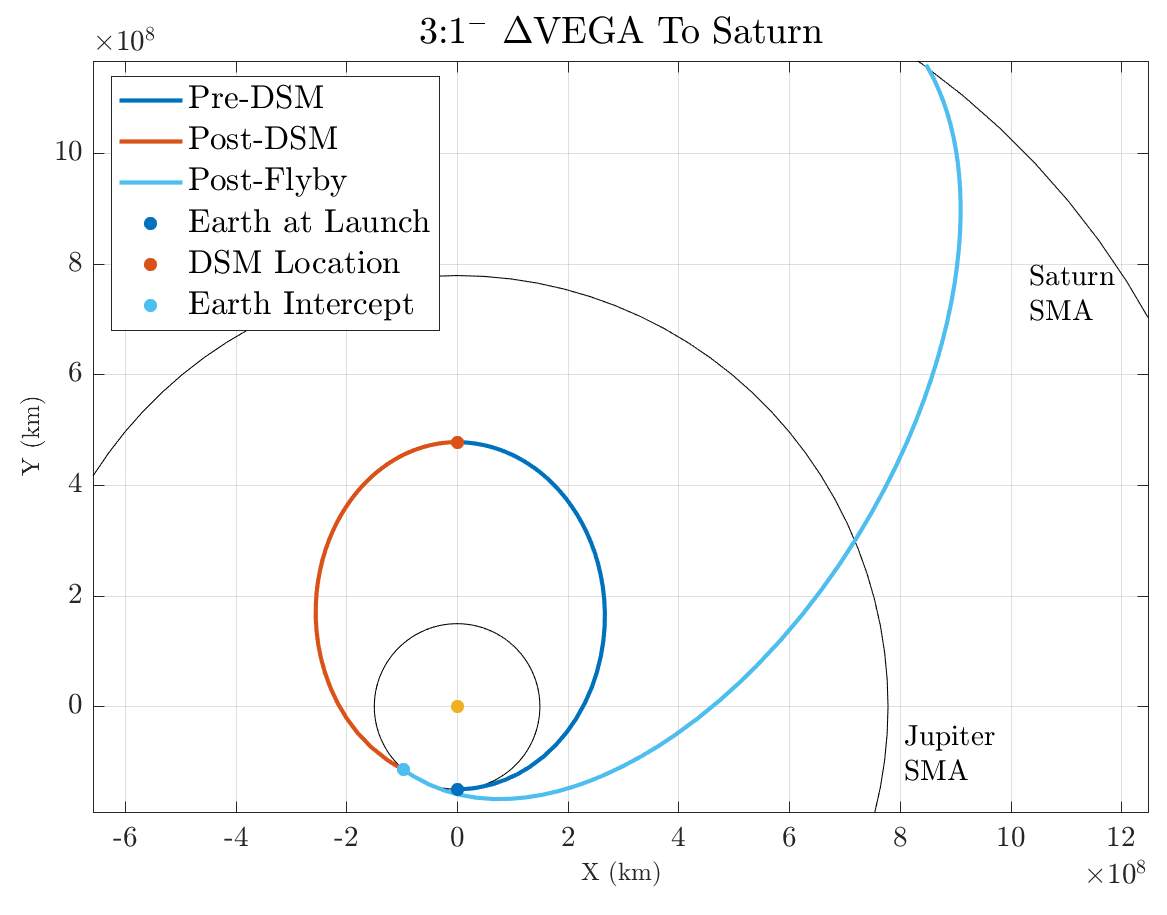
\includegraphics[width=3.6in]{./Figures/dsmmatlab}
	\caption{Example of a computed 3:$1^{-} \Delta$VEGA trajectory with a final aphelion radius roughly that of Saturn's semi-major axis. The launch $V_\infty$ is 6.97 km/s and the required DSM $\Delta$V is 0.39 km/s. The EGA flyby altitude was constrained to 200 km, which yielded the highest post flyby energy.}
	\label{fig:dsmmatlab}
\end{figure}
%
\\A Lambert arc is computed between these points and the resulting initial velocity change is used to find the DSM vector. The final velocity vector is assumed to be the heliocentric velocity of the leveraging orbit at the EGA. The relative velocity, $\vec{V_\infty}$ is computed and a planar flyby of Earth can now be calculated from the tree search algorithm. Fig.~\ref{fig:dsmmatlab} illustrates an example leveraging orbit being calculated for $\theta_{E}$ = 40.$7^{\circ}$. An energy maximizing flyby and propagation to the new aphelion is added to the end of the $\Delta V$EGA orbit to show the resulting trajectory.
\\\indent From testing, we noticed that as $\mid\theta_E\mid$ increased, a normal component of the DSM $\Delta$V appeared and grew larger. To limit the $\Delta$V to only a tangential component, and in return to reduce the total $\Delta$V required, a minimizer can be employed. This optimization comes at the expense of a higher launch energy and a longer flight time for trajectories requiring large $\mid\theta_E\mid$. Differing trends from Sims et. al. analysis of $V_\infty$ leveraging\cite{sims1994} were only noticed in high total $\Delta$V cases for each $k$ leveraging orbit family. These solutions were discarded from the lookup table due to delivering lower aphelion radii post-flyby when compared to lower total $\Delta$V leveraging orbits of the same family. The case presented in Fig.~\ref{fig:dsmmatlab} is intended to matche that discussed by Sims et. al\cite{Sims1997} and has nearly identical results. The inclusion of deep space maneuvers, not specific to $\Delta V$EGAs, are not implemented in the current form of the tree search. However, because the algorithm patches the two conics forming the leveraging orbit using the Lambert's method, the possibility to extend DSM maneuvers for off-tangent $V_\infty$ departures and targeting for the flyby can be implemented. This inclusion adds another dimension to the lookup table but offers leveraging maneuvers between Earth and Venus.
\\\indent Now that the $\Delta V$EGA orbit properties are known, the lookup table solution can be extended to the actual solar system model in the tree search. The table values are represented in a relative frame with respect to Earth's state vector at the launch epoch. A subsequent transformation of the departure velocity and pre-EGA incoming $\vec{V_\infty}$ can be done in order to find their specific components corresponding to an Earth epoch in the Ecliptic J2000 frame. From the initial node in the tree, a set of Earth leveraging time-of-flight nodes are created corresponding to their respective $k$ and $\theta_E$ parameters. The number of these leveraging nodes included in the initial flight time layer of the tree is directly related to the angular spacing of $\theta_E$. As the resolution becomes finer, by increasing the $\textit{detail}$ input to the search, the estimated $\Delta$V becomes more accurate. This, however, increases of the number of tree nodes created, and so for a rough idea of the trajectory search space, a coarse resolution is preferred. The discontinuous $\Delta$V post-EGA required to patch the incoming leg from the leveraging orbit and outgoing leg to the next planet node will determine if the leveraging node and its performance is effective for the transfer. Using this method, a distinction between the $\Delta V$EGA trajectory families to different outer planets can be observed.


% Force the text below to next page
\phantom{p. 1}
\clearpage



\subsection{Case 3: $\Delta V$EGA Opportunities to Neptune via Jupiter}
The tree search algorithm can now be extended to an exploratory context to find possible trajectories. With the interest in icy moon exploration in the solar system, a sequence to Neptune, and in return Triton, is explored\cite{Hubbard2010}. An arbitrary launch period was selected for this evaluation, and the search is limited to trajectories with the inclusion of a $\Delta V$EGA to evaluate its integration and performance. The number of iterations was set at 10,000 as this is seen to have a good compromise between calculation time and the number of search results. For a sequence to Neptune, it is desired to have a higher incoming relative velocity at Jupiter in order to have the appropriate outgoing energy to reach Neptune. With this in mind, the intent of the search was to find $\Delta V$EGA trajectories that deliver a high post EGA semi-major axis so the encounter velocity is maximized. The $\textit{detail}$ option is set to 16 which creates 8 $k$:1$^{-}$ and $k$:1$^{+}$ nodes for each $k$ family. This spread is seen to balance the computation time, due to the number of nodes created, and the accuracy of the DSM's $\Delta$V estimate. The launch C3 is set to explore the possibility of 2:1 $\Delta V$EGAs and the 3 and 4 $k$ leveraging families  would include the additional required velocity in the unoptimized $\Delta$V. The angular dispersion was set to 22 degrees yielding a fairly dense search space solution set. The results of the input search space are summarized in Table~\ref{tab:tritonInputs}:
%
%
\begin{table}[h]
    \begin{center}
        \caption{Inputs for $\Delta V$EGA Trajectories to Neptune via Jupiter}
        \label{tab:tritonInputs}
        \begin{tabular}{l|c}
					\toprule
            \textbf{Input Name} & \textbf{Input Value}\\
            \hline
            Arrival Planet & Neptune \\
            Launch Window \quad \quad & Jan 01, 2029 --- Jul 01, 2029 \\
            Iterations & 10,000 \\
            $\Delta V$ Budget & 4.5 $\sfrac{km}{s}$ \\
            Max C3 & 35 $\sfrac{km^2}{s^2}$ \\
            Detail ($d$) & 16 \\
						\bottomrule
        \end{tabular}
    \end{center}
\end{table}
%
%
%
\begin{figure}[ht]
	\centering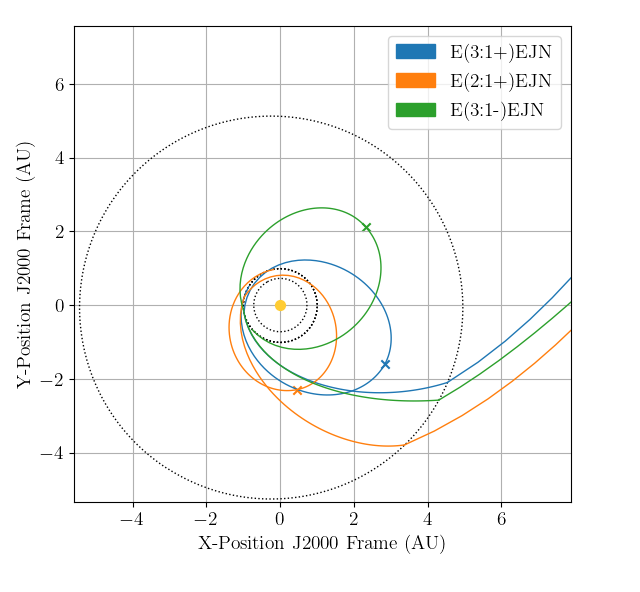
\includegraphics[width=3.6in]{./Figures/tridentMCTS}
	\caption{Different resulting E($\Delta$V)EJN sequence types from the search. The outermost dashed line is the semi-major axis of Jupiter, the middle dashed line is Earth's, and the innermost is Venus's. The $\Delta V$EGA type is labeled above and the mark on the leveraging orbit denotes the approximate DSM location.}
	\label{fig:tridentMCTS}
\end{figure}
%
%
\\\indent The search completed in 700 seconds and resulted in 1,714 sequences from the 178,545 nodes created. As expected, most solutions used the 2:1 or 3:1 leveraging maneuvers, and a few 4:1 and direct EJN sequences were found with large unoptimized $\Delta$V values. Fig.~\ref{fig:tridentMCTS} shows three different $\Delta V$EGA sequence types that comprise a majority of the search results. It is important to note that the 2:1$^{-}$ trajectories were not found in the search space due to not being able to deliver sufficient $V_\infty$ to Jupiter to continue onto Neptune. The 2:1$^{+}$ trajectories have long duration flight times (in excess of 17 years) which is expected due to the relatively low heliocentric energy flyby of Jupiter compared to other leveraging orbit families. Table~\ref{tab:tritontop25} lists the top 25 trajectories from the sequence that minimize the unoptimized $\Delta$V. Several 3:1 cases appeared in the results which reduce the flight time to Neptune to around two thirds the time (13 years) 
%
%
\\\indent For the optimization process, all initial guess conditions were taken from the tree search output and following bounds were set: plus or minus 30 days for the Earth launch, flyby, and DSM epochs and plus or minus 100 days for the Jupiter and Neptune encounter epochs. The maximum launch $V_\infty$ was allowed to be 0.01 $km/s$ over the predicted requirement from the search, and the limits on the DSM $\Delta$V were plus or minus 0.3 $km/s$ from the estimated value from the used lookup table solution. Fig.~\ref{fig:maltotriton} shows examples of two optimized trajectories resulting from the search. The left plot is an example of a 2:1$^{+}$ $\Delta V$EGA which requires a launch $V_\infty$ magnitude of 5.39 $km/s$ (as opposed to the 5.38 $km/s$ from the prediction). The 2:1 leveraging trajectory has an incoming $V_\infty$ to Jupiter of around 8 $km/s$ which yields a 6400 day flight time to Neptune. Though the trajectory has a relatively low Neptune arrival velocity (around 7.8 $km/s$), making it a good candidate for a capture, the flight time makes the mission considerably longer than the 3:1 solution. The case presented utilized an intercept $\theta_E$ of 42 degrees which has an estimated DSM $\Delta V$ of 0.43 $km/s$, and the optimizer's computed $\Delta$V is 0.55 $km/s$. Because the tree search selects evenly spaced nodes between a range of $\theta_E$ values, it is likely to under or overestimate the required maneuver magnitude. The optimizer is able to move the DSM epoch, account for flyby targeting, and the subsequent intercept true anomaly, further introducing variance in the required $\Delta$V. The 3:1 case in Fig.~\ref{fig:maltotriton} (right side) has a launch $V_\infty$

Both cases reach a bounded value, denoted by the parenthesis around the TOF at Neptune, and this likely due to dates shifting from the initial conditions.
%
%
\begin{figure}[ht]
		\centering
		\begin{minipage}{0.50\textwidth}
				\centering
				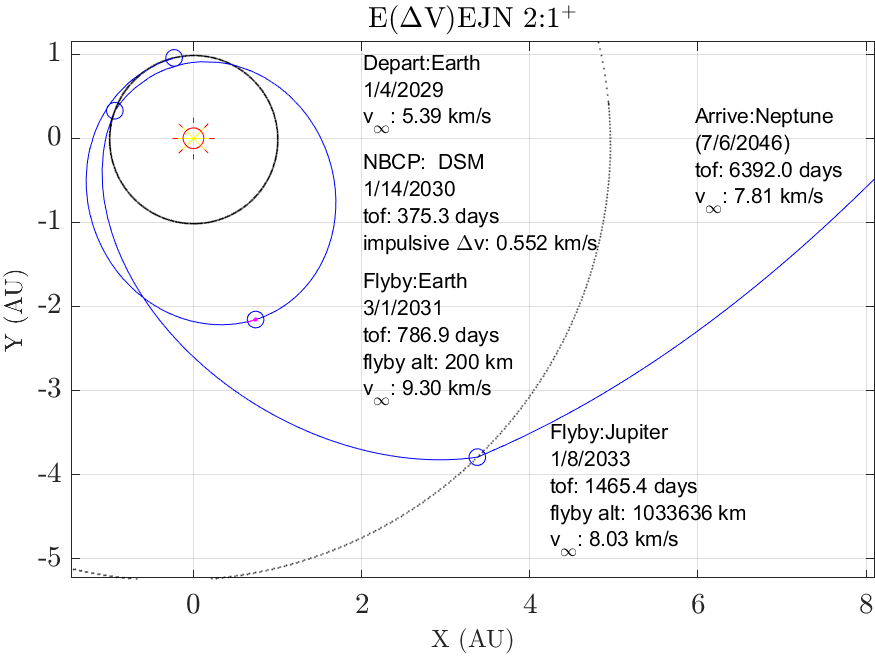
\includegraphics[width=1.0\textwidth]{./Figures/eejn21plus}
    \end{minipage}\hfill
		\begin{minipage}{0.50\textwidth}
				\centering
				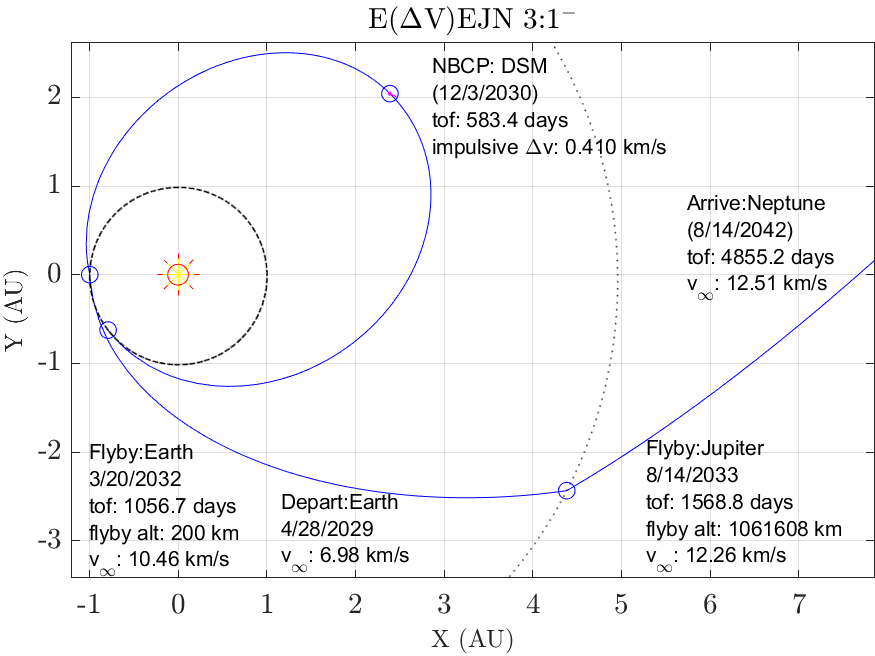
\includegraphics[width=1.0\textwidth]{./Figures/eejn31minus}
		\end{minipage}
		\caption{Optimized trajectory examples from the search. The left plot is an example of a 2:1$^{+}$ and the right is a 3:1$^{-}$. The 2:1$^{+}$ is able to reach Neptune with a much lower $V_\infty$ due to a slower relative velocity into Jupiter when compared to the 3:1$^{-}$ sequence.}
		\label{fig:maltotriton}
\end{figure}
%
%
\\$\textbf{Need to add discussion on leveraging performance}$
The deep space maneuver magnitude and direction vary from the search results due to various factors. The optimization process takes into account the change in declination for the outgoing flyby and so depending on the transfer, an additional Z-component of velocity is added by the optimizer to target the appropriate Earth flyby B-Plane angle. Another source of discrepancy is in the maneuver location. In the lookup table, the assumption is that the deep space maneuver is conducted at the aphelion of the leveraging orbit. In practice, the maneuver can be shifted before of after by the optimizer. Table~\ref{tab:} summarizes a few optimized cases and their predicted DSM $\Delta$V versus the calculated value from the optimization process.


The search returns several cases of interest which have been optimized and shown in Fig.~\ref{fig:maltotriton1} and Fig.~\ref{fig:maltotriton2}. Sequences that utilize a 2:1$^{-}$ and 2:1$^{+}$ have the lowest launch energy, but also have fairly large deep space maneuvers. The
\\$\textbf{THIS PART IS NOT DONE YET}$



\clearpage
\noindent $\textbf{Notes}$
\\
\\\noindent Intro
		\\-We can remove the machine learning paragraph. We already mention the alg is heuristic free.
		\\-Should we mention rosetta if we don't prove it in the test cases?
		\\-Add a work scope (In this paper we are going to do ...)
\\
\\\noindent Theory
    \\-Theory $e_{out}$ needs to be defined in words (I assume its eccentricity from eq8)
		\\-Sentence starting with "Using the Newton..." is a fragment
		\\-"real life" under equation 9
		\\-"fuel usage" should be reworded?
		\\-comparing energy and vinf together (select 1 or the other)
		\\-DSM theory I use "we" but we dont really use we anywhere else in the theory
\\
\\\noindent Test Cases
		\\- maybe reword "no basis for its astrodynamics" (In order to test the algorithm's performance and ability to return useful sequence pairs...)
		\\-"Europa Clipper's" 3rd sentence in Performance Evaluation
		\\-push limits of powered flyby?
		\\-we can remove the "trident" name for Neptune trajectories bc they are not using EEVEE sequences.
		\\-The first case is a search to find a sequence similar to Europa Clipper's interplanetary trajectory (15F9-A22 EEVEEJ) utilizing multiple gravity assists of Earth and Venus to reach Jupiter[source].
		\\-maybe we should include a reminder of what d means?
		\\-"1.9 billion possible combinations possible..." reword
		\\-For Table 2 we should mention its dates for Europa Clipper and not Galileo in the caption.
		\\-After table 3, "An additional constrain"
		\\$<$got up to Figure 5$>$
		\\
	  \\-label for Table 8 in appendix to reference in text (I am using ref tab:tritontop25  right now in the text)


\phantom{p. 1}
\clearpage
\bibliographystyle{./AAS_publication}
\bibliography{./referencesDSMSsection}

\end{document}
